%
% fig-unterzyklen.tex
%
% (c) 2025 Prof Dr Andreas Müller
%
\begin{figure}
\centering
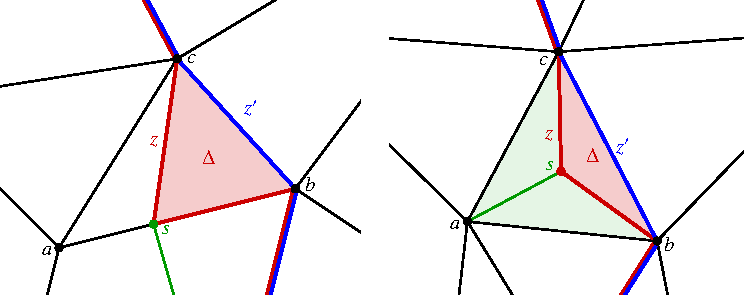
\includegraphics{chapters/120-topologie/images/unterzyklen.pdf}
\caption{Unterteilung eines Zellenkomplexes mit einem neuen Punkt $s$
auf einer Kante (links) bzw.~im Inneren (rechts) eines 2-Simplex.
Ein Zyklus $z$, der die neue Kante $cs$ verwendet, verwendet auch eine der
neuen Kanten $as$ oder $sb$ ($sb$ im gezeichneten Fall).
Subtraktion des Randes von $\Delta$ verwandelt $z$ in $z-\partial\Delta = z'$.
$z$ und $z'$ sind daher homolog, der Zyklus $z$ ist keine neue
Homologieklasse.
\label{buch:topologie:simplex:fig:unterzyklen}}
\end{figure}
